%% LaTeX2e class for student theses
%% sections/content.tex
%% 
%% Karlsruhe Institute of Technology
%% Institute for Program Structures and Data Organization
%% Chair for Software Design and Quality (SDQ)
%%
%% Dr.-Ing. Erik Burger
%% burger@kit.edu
%%
%% Version 1.3.3, 2018-04-17

\chapter{Our Algorithm}
\label{ch:alg}

The algorithm and the underlying acceleration data structure we chose is inspired by the tree construction and traversal algorithm of the bounding volume hierarchy. Similarly to the BVH, we will construct a binary tree before rendering, and traverse through the tree to find the appropriate light when we are given the point of the intersection in the scene. Analogous to most BVH algorithms, our light BVH construction runs on a single thread, while the traversal can run on concurrent threads. Since the construction of the tree only a small fraction of the rendering time, this does not pose a problem even on scenes with over one million light sources.

\section{Informal Description of the Algorithm}
\label{sec:alg:idea}

In this section we will give rough overview of the ideas of our algorithm. We have thought about jumping straight into the in-depth implementation part and skipping the informal description of the algorithm but some parts of the implementation decisions are hard to understand without having at least a rudimentary overview of the algorithm. For instance, when we talk about the information every node of the tree needs to store, it is much easier for the reader to comprehend our train of thought when he has a general idea how our tree traversal algorithm works.

First, when we have access to all of the light sources of the scene, we want to create a binary tree data structure that includes every single light source of the scene. We call our tree the light bounding volume hierarchy (light BVH), because similarly to the BVH construction, we will also split the scene spatially parallel to coordinate axis. We will also use a heuristic to find the best split of all three dimensions, comparable to the surface area heuristic. Our heuristic, the surface area orientation heuristic (SAOH) has some crucial difference to the SAH. First, instead of amounting the number of primitives, we will factor in the total emission power of the lights. Second, we have added an orientation factor. This orientation factor tries to keep light sources with similar orientations in the same node. This way, we have split the branches so different orientations most likely branch to different children of the tree and thus, finding the more likely child when traversing through the light BVH later will be clearer. When we have a node with only a single light source, this node is a leaf.

After we have constructed our light BVH, the next step would be traversing through the tree when we want to sample a light given an intersection point. Obviously, we don't just want to return a random light source which would make this algorithm pointless, but instead we want to importance sample a light that has most likely a strong contribution to the point. Therefore, we will define an importance measure for every node given the intersection point, that factors in the distance between the point and the node, the emission power of the node and an angle importance factor. We will start at the root of the light BVH and generate a uniform random number. Then, for every branch, a decision has to be made which child to take based on the importance measure and that random number. When we have arrived at a leaf node, that will be the light source we return.

What I have just described was our algorithm when we only want to sample a single light source. Conty and Kulla have shown in \cite{MLS}, that there are situations, where it is desirable to sample multiple light sources for one intersection point. That is the reason why we allow the user to define a split threshold. Based on the split threshold and a score which we calculate for every branch, instead of sampling only the left or the right child, we will sample both nodes. At the end, return one or multiple sampled lights. Afterwards, the sampled lights are used for the path tracing algorithm.

\section{Own Data Structures}
\label{sec:alg:ows}

In this section we will be discussing our own data structures. We will show our internal representation of our data structures now and reason why they are represented like this.

\subsection{Bounds\_o}

\begin{figure}
	\begin{center}
		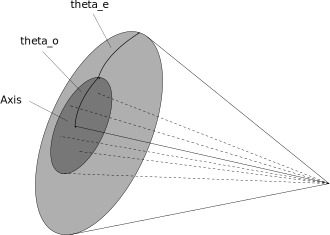
\includegraphics[width=0.3\textwidth]{bounds_o.png}
		\caption{Our internal representation of the Bounds\_o struct}
		\label{fig:boundso}
	\end{center}
\end{figure}

First we will introduce the Bounds\_o struct (\ref{fig:boundso}). This struct represents the orientation bounds of a certain light source or a whole node. For a single light, the axis defines the orientation direction of the light source, while for a node, the axis represents the interpolated axes of all light sources included in the node. Theta\_o defines the maximum angle between the axis of the node and any light source included in this node. Theta\_e defines the additional emission range added to theta\_o for spotlights or area light sources. How we have pictured the geometric representation can be seen in \ref{fig:boundsogeo}. In our implementation, we accept point lights, spotlights and area light sources as light sources. This is how we initialize the Bounds\_o struct for single lights:

\begin{itemize}
	  \setlength\itemsep{0em}
	\item Point light
	\begin{itemize}
		  \setlength\itemsep{0em}
		\item Axis = (1, 0, 0)
		\item theta\_o = $\pi$
		\item theta\_e = $\pi/2$
	\end{itemize}
	\item Spot light
	\begin{itemize}
		  \setlength\itemsep{0em}
		\item Axis = spot direction
		\item theta\_o = 0
		\item theta\_e = spot's apperture
	\end{itemize}
	\item Area light
	\begin{itemize}
		  \setlength\itemsep{0em}
		\item Axis = normal of the geometric representation
		\item theta\_o = 0
		\item theta\_e = $\pi/2$
	\end{itemize}
\end{itemize}

\begin{figure}
	\begin{center}
		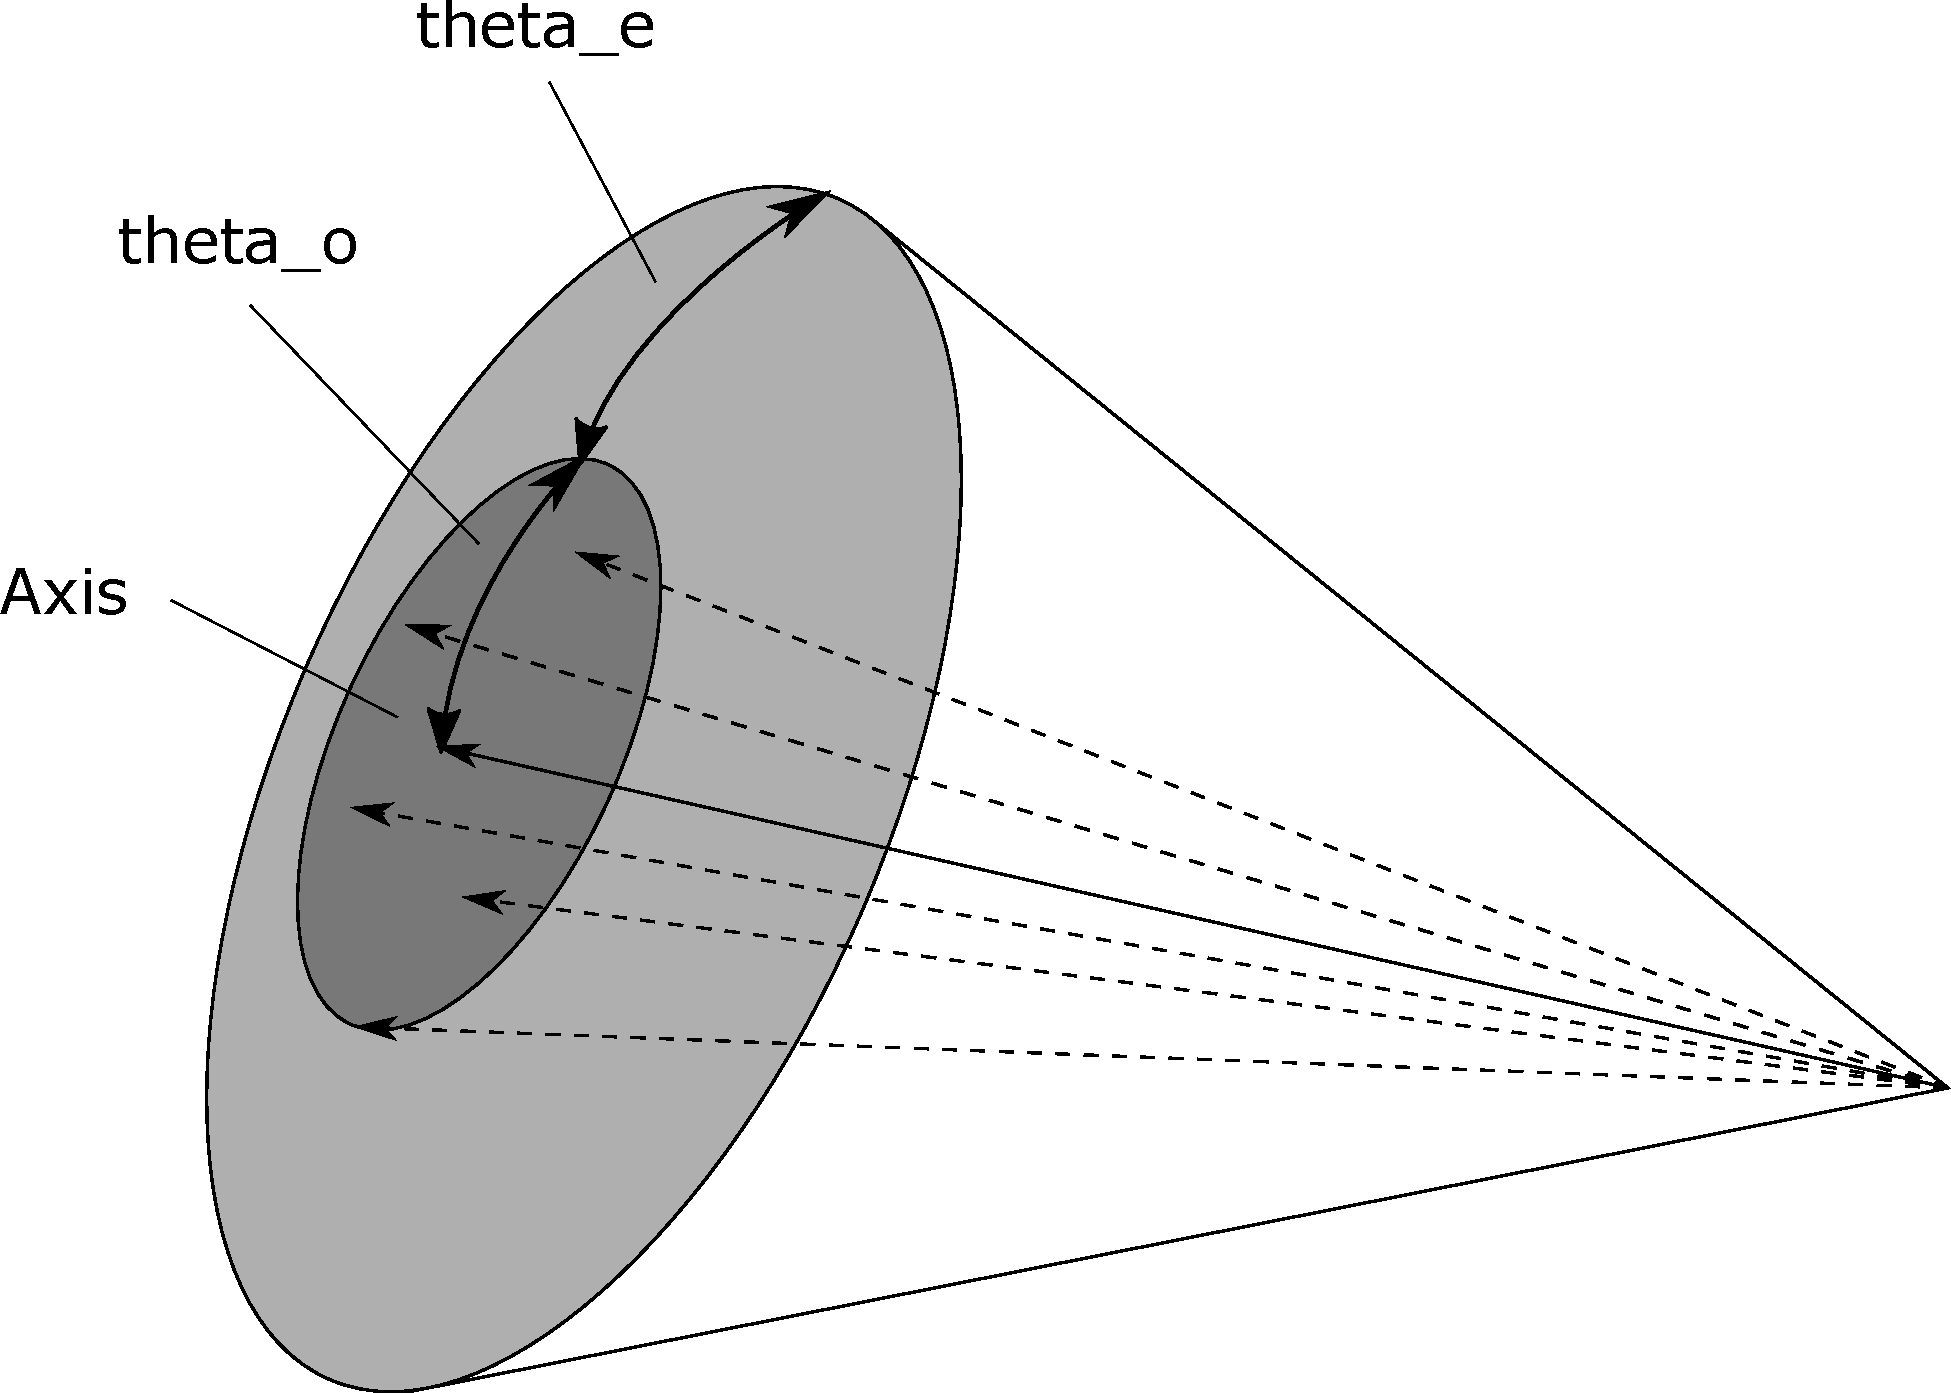
\includegraphics[width=0.6\textwidth]{bounds_o.pdf}
		\caption{geometric idea of the Bounds\_o struct}
		\label{fig:boundsogeo}
	\end{center}
\end{figure}

\subsection{Node representation}

We used two different implementations to represent a node in our light BVH tree (\ref{fig:lightbvhnode} and \ref{fig:linearlightbvhnode}). Both implementations are very similar, containing the two bounding bounds $bounds_w$ for the world space bounds and $bounds_o$ for the orientation bounds, as well as other other information that we will need for the tree traversal later. $Energy$ defines the combined energy of the lights under this node, $nLights$ describes the number of lights under this node, $centroid$ stores the centroid of the world space bounds, and $splitAxis$ stores the coordinate axis that splits the two children of this node. 

The main difference between the two implementations is the way to access the children of the nodes. In our $LightBVHNode$, we have explicit pointers to the two children, while we define the children implicitly in out $LinearLightBVHNode$. Since all of our $LinearLightBVHNodes$ are stored in aligned memory, the way we access the left child is just by incrementing the pointer of the current $LinearLightBVHNode$ by 1. The index needed to access the right child is stored in $secondChildOffset$. To access the second child, we just add $secondChildOffset$ to the base pointer of the root of the tree. If the node is a leaf of the tree and thus only contains one light source, $lightNum$ stores the index of that light source in both implementations.

\begin{figure}
	\begin{center}
		\includegraphics[width=0.5\textwidth]{lightbvhnode.png}
		\caption{Our internal representation of the LightBVHNode struct}
		\label{fig:lightbvhnode}
	\end{center}
\end{figure}

\begin{figure}
	\begin{center}
		\includegraphics[width=0.4\textwidth]{linearbvhnode.png}
		\caption{Our internal representation of the LinearLightBVHNode struct}
		\label{fig:linearlightbvhnode}
	\end{center}
\end{figure}

\section{Surface Area Orientation Heuristic}
\label{sec:saoh}

We have mentioned that we use a different splitting heuristic to build our tree as opposed to using the SAH in a BVH. But we do follow a similar main idea to split the primitives (in our case, the lights) parallel to a coordinate axis, which means that we split in world space. Comparable to splitting the BVH with SAH, where the goal is to minimize the cast of traversing a branch combined with the probability of hitting it, we want to minimize the probability of sampling a branch here. Also, instead of only regarding the number of primitives for each branch, we will rather take into account the combined energy of all the light sources of each branch. Equivalently to SAH, we will also include the surface area in our calculations. So while we do split in world space, we will use the orientation bounds, along with the surface area and the energy, to determine the quality of a certain split. In summary, we define the probability of sampling a given cluster $C$ in the surface area orientation heuristic for as:

\begin{equation}
P(C) = M_A(C) * M_\Omega(C) * Energy(C),
\end{equation}

$M_A(C)$ being the surface area of the cluster, $M_\Omega(C)$ being the bounding cone measure. The surface area of a clusters bounding box with length $l$, width $w$ and height $h$ is the sum of its six faces:

\begin{equation}
M_A(C) = 2(lw + wh + hl).
\end{equation}

We used a weighted definition for our bounding cone measure. Remember that we have defined $\theta\_o$ as the bounding angle that encloses the orientation vectors of all the light sources in the cluster, while $\theta_e$ describes their emission range. Obviously, the cone enclosed with $\theta_o$ will most likely have a greater in emission power and thus, we will weight the volume confined by $\theta_o$ with a cosine. The measure we have used and has been described in \Cite{MLS} is as follows:

\begin{equation}\label{eq:cone}
M_\Omega(C) = 2\Pi * \bigg[(1-\cos(\theta_o)) + \int_{\theta_o}^{\theta_o + \theta_e}\cos(\omega - \theta_o) * sin(\omega)d\omega\bigg]
\end{equation} 

TODO:Zeichnung

Then, we describe the quality of a split as:

\begin{equation}
c(C_{left}, C_{right}) = \frac{P(C_{left}) + P(C_{right})}{P(C)}.
\end{equation}

Consequently, the quality of a split is inverse to its cost:

\begin{equation}
q(C_{left}, C_{right}) = \frac{1}{c(C_{left}, C_{right})}.
\end{equation}

It is important to note that our heuristic tries to find out the possible split in all three dimensions with the given cluster. Therefore, we will try to find the split with the highest quality and split the cluster there.

\section{Light Bounding Volume Hierarchy Construction}
\label{sec:alg:con}

In this section we will be talking about our in-depth implementation of the tree construction. The tree constructor method takes two parameters. First, a vector containing all the light sources in the scene. Second, we will take a parameter defining the split threshold that describes if we want to sample multiple light sources when traversing the light BVH later (\ref{subs:split}). The split threshold is a normalized value between 0.0 and 1.0. A split threshold of 1.0 never splits, we would only shade one light per point and a split threshold of 0.0 always splits, which means all lights of the scene are shaded. Note that our algorithm is implemented to work with any combination of point light sources, area light sources and spotlights.

\begin{algorithm}
	\caption{LightBVHAccelerator constructor}
	\label{LightBVHAccelerator}
	\begin{algorithmic}[1] % The number tells where the line numbering should start
		\Procedure{LightBVHAccel}{vector<Light> lights, float splitThreshold}
		\State $LightBVHNode \; *root  \gets recursiveBuild(lights, 0, lights.size());$
		\State $LinearLightBVHNode \; *nodes \gets AllocAligned(totalNodes);$ 
		\State $flattenLightBVHTree(nodes, root, 0);$
		\EndProcedure
	\end{algorithmic}
\end{algorithm}

The $lightBVHAccel$ constructor initializes the tree construction. First, we will be using a recursive approach to build the light BVH. We will pass the light sources of the scene in an array and the starting and ending indices of the current node, obviously for the root of the light BVH we will pass the whole range of our vector. Then, after we have constructed our tree represented by $LightBVHNode$ objects, we will flatten the tree in a compacter form represented by $LinearLightBVHNode$ objects to ensure that our tree requires as little memory as possible and to improve cache locality. $Nodes$ will later be our object to run our tree traversal on.

\begin{algorithm}
	\caption{LightBVHAccelerator recursive build}
	\label{recursiveBuild}
	\begin{algorithmic}[1] % The number tells where the line numbering should start
		\Procedure{recursiveBuild}{vector<Light> lights, int start, int end}
		\State LightBVHNode *node;
		\If{end - start == 1}
			\State *node = $initLeaf()$;
			\State \Return node;
		\EndIf
        \ForEach {\texttt{dimension}}
        	\State <calculate axis and thetas for the whole node for current dimension>
			\State <calculate all split costs for current dimension>
		\EndFor
		\State <find out best split>
		\State *node = $initInterior(recursiveBuild$(leftChild), $recursiveBuild$(rightChild)); \\
		\Return node;
		\EndProcedure
	\end{algorithmic}
\end{algorithm}

Our implementation of the light BVH construction can be split into multiple sections. Obviously, we want to cover the base case first, when we only have a single light source under the node. In this case, we cannot split further, so we will just initialize a leaf node with the one light source and return this leaf node. 

\subsection{Axis Calculation}
\label{subs:axis}

Next, we will do axis calculations for the whole cluster for a specific dimension. We have tried two different approaches for the axis calculations. Our first approach used the median of the individual axes of all lights included in the cluster sorted by the specific dimension we are working on. So, if we wanted to find out the qualities of the individual splits if we split the lights at a particular x-coordinate, we would take the axis of the median light if we sorted them according the x-coordinate of their axes. This approach leads to a major problem. Since our geometric representation is three-dimensional, taking the median axis sorted by a single dimension does not always represent the ideal axis that we are looking for. Suppose we have a scene as modelled in \ref{TODO}. TODO: Zeichnung Beschreibung

TODO:Zeichnung

Our second approach that we are using now deals with this problem properly. Instead of using the median axis, we use the average or the normalized sum of the individual axes of all light sources in the cluster:

\begin{equation}
C_{axis} = \frac{\sum_{i = 0} a_i}{|\sum_{i = 0} a_i|},
\end{equation}

with $a_i$ being the axis of the i-th light source in the cluster. This axis definition for a cluster eliminates the problem presented in \ref{TODO}. Both median and average calculations have $O(n)$ time complexity, but especially in scenes with symmetric objects that represent light sources, our current approach leads to much better results.

\subsection{Theta Calculations}
\label{subs:theta}

\begin{algorithm}
	\caption{Theta calculations}
	\label{thetacalculations}
	\begin{algorithmic}[1] % The number tells where the line numbering should start
		\Procedure{calculateThetas}{vector<Light> \$lights, 3DVector axis, float *theta\_o, float *theta\_e}
		\For{\texttt{int i = 0; i < vector.$size$(); i++}}
			\State Light l $\gets$ lights[i];
			\State float current\_o $\gets$ 0.f;
			\State float current\_e $\gets$ 0.f;
			\If{(current\_o $\gets$ $radianAngle$(axis, l.axis) + l.theta\_o) > *theta\_o}
				\State *theta\_o $\gets$ current\_o;
			\EndIf
			\If{(current\_e $\gets$ current\_o + l.theta\_e) > *theta\_e}
				\State *theta\_e $\gets$ current\_e;
			\EndIf
		\EndFor
		\State *theta\_e -= *theta\_o;
		\State *theta\_e $\gets$ $min$(*theta\_e, $\Pi$ - *theta\_o);
		\EndProcedure
	\end{algorithmic}
\end{algorithm}

TODO: this code is shit wtf dude

We have listed our the calculations for $\theta_o$ and $\theta_e$ in \ref{thetacalculations}. The procedure takes the base address of a vector containing of the lights that define the specific cluster, as well as the axis of the cluster. Also, pointer to two floats are passed to return the $\theta$-values. The calculations made are very simple; we iterate through the lights that were passed to us and calculate the individual $\theta_o$ and $\theta_e$ values of the given axis with the axis of the whole cluster. If any of the $\theta$ values are greater than the current maximum $\theta$ values we have stored, we update our maximum $\theta$ values. At the end, when we have processed all light sources, we have to first subtract $\theta_o$ from $\theta_e$ as we only store the additional angle to $\theta_o$ in $\theta_e$. Next, we will also need to limit $\theta_e$ with $\Pi - \theta_o$, otherwise it is possible to get a negative integral in our bounding cone measure \ref{eq:cone}. This is something we want to avoid because the measured volume of the bounding cone should always be non-negative.

\subsection{Buckets}
\label{subs:buckets}

Before we jump into our split cost implementation, we want to talk about a design decision we made. The first approach we tried was to split the light sources after every single light source, which means, if we had 1.000 lights, we would have 999 different splits in each dimension. We realized that this approach does not scale well for very large amounts of light sources. We measured the time for building the light BVH on different scenes with varying amounts of emitters on a computer with a Intel® Core™ i7-4770K processor and 16 gigabyte of main memory. For instance, a scene with 10.000 emitters works just fine with a rendering time of TODO. On the other hand, the tree construction time of another scene with one million light sources takes TODO. Obviously, this construction time is way too long and not useful for practical uses. 

TODO: Zeichnung 

Therefore, we decided to use specific amounts of buckets that determine the position where we split the light sources. At the start, we will define a maximum amount of splits that we want to calculate for any cluster. What has worked well for us is to calculate a maximum number of 10.000 splits. This way, we have an acceptable rendering time of TODO for the scene with one million light sources, while the split quality stays roughly the same like if we would calculate every possible split. When we have settled on $b$, the amount of buckets to use, we will define the number of light sources in each bucket as:

\begin{equation}
n = \frac{b}{N},
\end{equation}

with $N$ being the total number of emitters of the cluster. Then, we will split the lights of the cluster at the indices that are multiples of $n$, resulting to $b$ different splits.

\subsection{Split Cost Calculation}
\label{subs:splitcost}

\begin{algorithm}
	\caption{Split Cost Calculation}
	\label{alg:splitcostcalculation}
	\begin{algorithmic}[1] % The number tells where the line numbering should start
		\Procedure{calculateCost}{vector<Light> \$lights, int buckets}
		\State float[buckets] cost;
        \ForEach {\texttt{split i}}
		\State <calculate axis, thetas, AABB and energy for the left part>
		\State <calculate axis, thetas, AABB and energy for the right part>
		\State <calculate leftCost, rightCost and totalCost>
		\State cost[i] $\gets$ (leftCost + rightCost) / totalCost;
		\EndFor
\State \Return cost;
\EndProcedure
\end{algorithmic}
\end{algorithm}

First, we have to sort the light sources by their coordinate value of the current dimension we are working on, since we split in world space. Then, we use the previously discussed buckets to determine positions where to split the emitters. For each individual split, we will be doing axis, theta and AABB as described in \ref{subs:axis}, \ref{subs:theta} and \ref{sec:aabb}. The total energy of a cluster is simply the sum of the energy values of the individual light sources. Afterwards, we will do the split cost calculations according to \ref{sec:saoh}.

\section{Light Bounding Volume Hierarchy Traversal}
\label{sec:alg:tra}

\subsection{Splitting}
\label{subs:split}